% !TEX encoding = UTF-8
% !TEX TS-program = pdflatex
% !TEX root = ../tesi.tex

%**************************************************************
\chapter{Azzurra Flow Engine}
\label{cap:flow engine}
%**************************************************************
\intro{Nel seguente capitolo verrà illustrato prima di tutto la struttura di un flusso conversazionale e successivamente il funzionamento del Azzurra Flow Engine la conseguente generazione dei messaggi da parte del bot Azzurre e dell'utente umano}\\

%*************************************************************

\section{Cos'è}
Un elemento cardine dell'architettura di \textbf{Azzurra} è \textbf{Azzurra Flow Engine}. Esso è un motore conversazionale in grado di ricevere in input flussi conversazionali, implementati attraverso file JSON, che risiedono nel database di \textbf{Azzurra.io}. Essi vengono mandati in input a \textbf{Azzurra Flow Engine} quando il bot \textbf{Azzurra} ne fa richiesta. Questi file sono codificati secondo una certa struttura fatta dai cosiddetti blocchi conversazionali e da altri campi che verranno illustrati in seguito. Tornando su \textbf{Azzurra Flow Engine} come scritto, riceve in input il file di conversazione in JSON e grazie ai metodi che ha disposizione è in grado di interpretare i file JSON ricevuti e generare i messaggi che il bot \textbf{Azzurra} deve fare visualizzare all'utente nella chat.

\section{Flussi di conversazione}
I flussi di conversazione o conversazionali sono degli elementi fondamentali per la conversazione tra il bot e l'utente umano. Essi sono delle configurazioni in JSON, dove ogni configurazione contiene un flusso di conversazione, e ogni flusso è un possibile ramo di conversazione che può essere fatto tra il bot Azzurra e l'utente umano. Ogni configurazione contiene perciò dei particolari comandi che permettono al bot di sapere quali messaggi deve mostrare all'utente umano e come comportarsi in base alle sue scelte. Ogni configurazione ha un \textbf{id} che contiene un codice univoco in modo tale da poter identificare ogni flusso di conversazione. Inoltre, l'esecuzione dei flussi di conversazione prevede che all'inizio ci sia l'esecuzione di un cosiddetto \emph{main flow}, in modo simile a come avviene per i programmi software, cioè c'è una funzione detta \emph{main} che viene eseguita per prima all'avvio del programma. Per indicare quale tra l'insieme dei flussi sia il \emph{main} si utilizza il campo \textbf{isMainFlow} dandogli il valore \emph{true}.
Oltre a questi campi esistono altri campi che sono:
\begin{itemize}
	\item \textbf{Shortcuts "shortcuts"};
	\item \textbf{Configurazione "config"};
	\item \textbf{Blocchi per la conversazione "blocks"}.
\end{itemize}
Tutti e tre verranno illustrati nelle seguenti sottosezioni.
\subsection{Shortcuts “shortcuts”}
Il campo \textbf{shortcuts} è il campo dedicato per le cosiddette "scorciatoie" cioè, tra le funzionalità che il bot offre all'utente c'è anche la possibilità di visualizzare un menu dove vengono mostrate tutte le funzionalità offerte dal bot e scegliere direttamente quelle eseguire in ogni momento.

\begin{figure}[htbp]
	\centering
	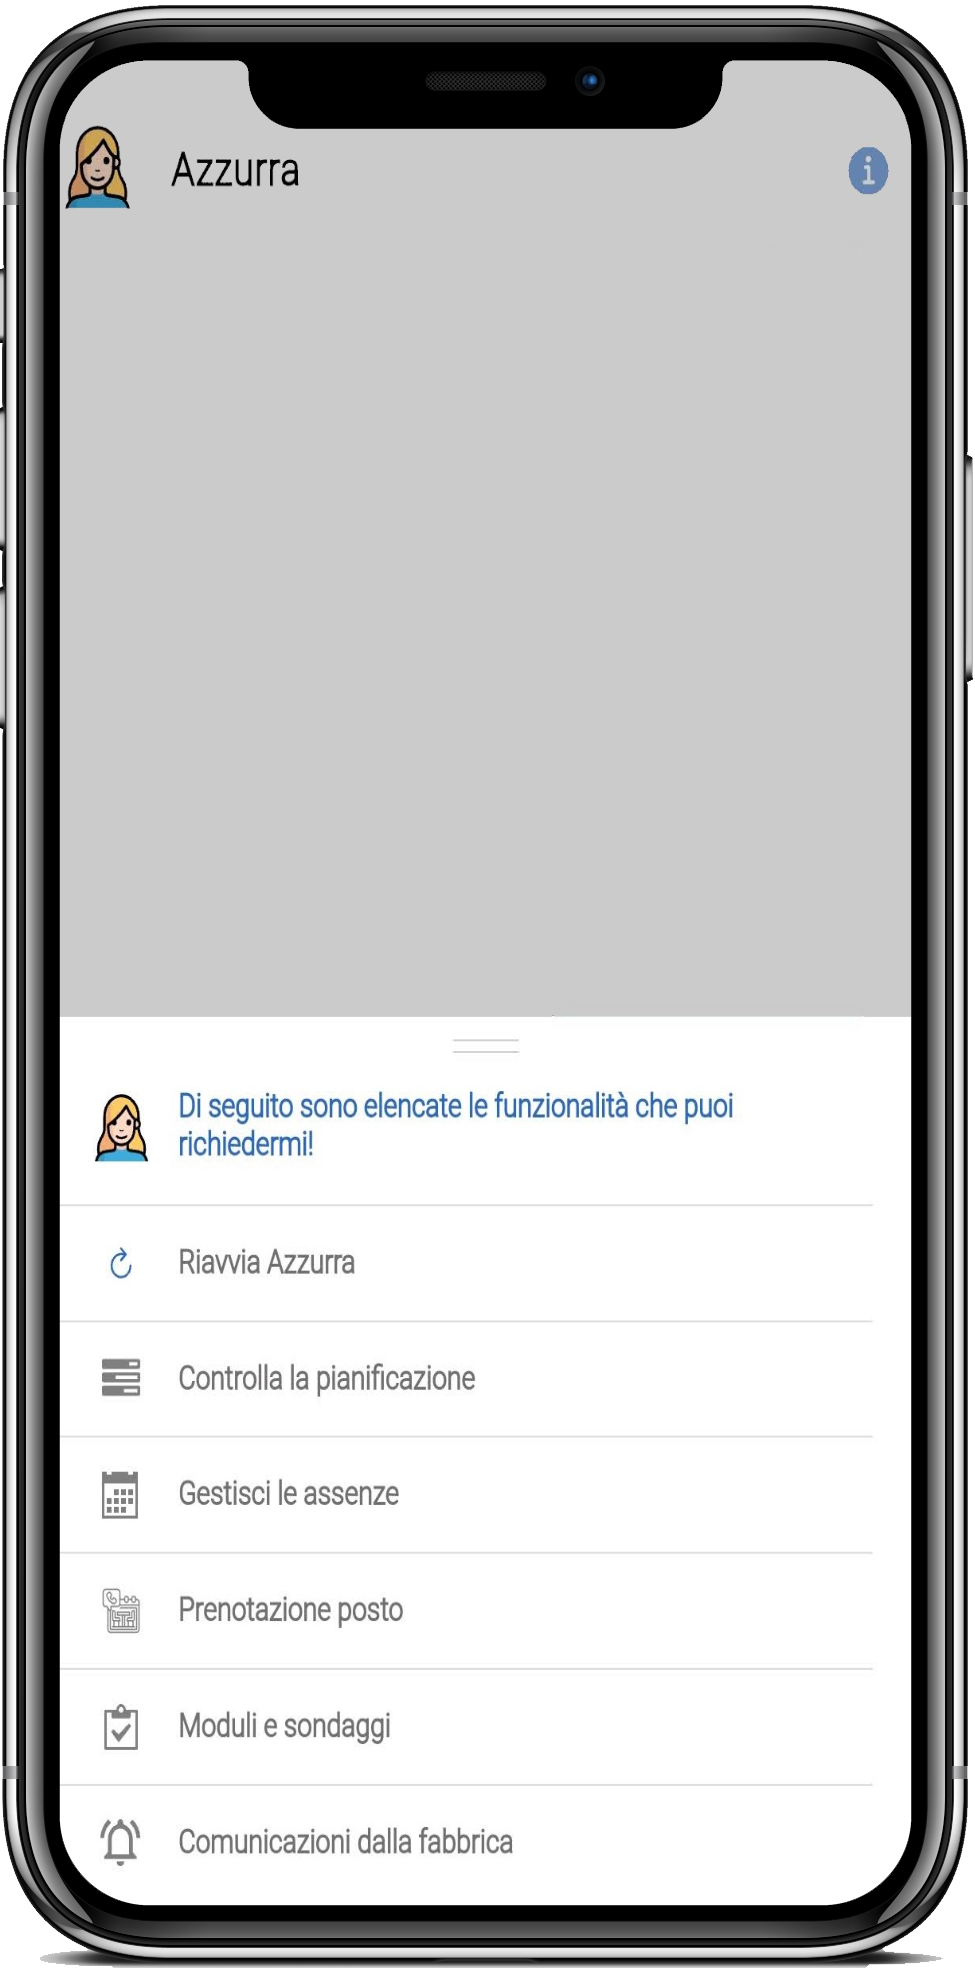
\includegraphics[scale=0.4]{shortcuts.PNG}
	\caption{Menu contenente le shortcuts disponibili}
\end{figure}

Il campo \textbf{shortcuts} viene indicato nel file con la \emph{keyword} \textbf{shortcuts}
e al suo interno contiene i seguenti campi:
\begin{itemize}
	\item \textbf{text}: È un campo che può essere di tipo \emph{string} e quindi contiene il testo da far visualizzare nel bottone della scorciatoia all'utente, oppure un oggetto che contiene un attributo per ogni lingua disponibile, dove ogni attributo ha il testo nella lingua straniera che l'attributo rappresenta. Il testo nella lingua di default (italiano) è contenuto nell’attributo “default” ;
	\item \textbf{flowId}: Contiene l'identificativo del flusso che la scorciatoia permette di far eseguire;
	\item \textbf{icon}: Per rendere la UI più accattivante è possibile aggiungere al bottone dedicato alla scorciatoia, delle icone per ogni scorciatoia.
\end{itemize}
\clearpage
\subsection{Configurazione "config"}
Il campo \textbf{config} permette di indicare attraverso il campo \textbf{startBlockId} quale blocco di conversazione del flusso deve essere eseguito per primo, per tale campo ci sarà il codice identificativo del primo blocco da eseguire. Il campo \textbf{configurazione} viene indicato nel file con la keyword \textbf{config}.

\subsection{Blocchi per la conversazione "blocks"}
Il campo \textbf{Blocchi} indicato nel file con la \emph{keyword} \textbf{blocks} contiene tutti i blocchi per la conversazione i quali indicano i messaggi che devono essere mostrati e i passi da eseguire a seconda delle scelte inserite dell'utente umano.
I blocchi utilizzati per la conversazione si differenziano tra lo loro dal tipo di blocco a cui appartengono. Ogni tipo ha proprie caratteristiche uniche ma anche delle caratteristiche comuni, questo perché tutti i tipi di blocchi per la conversazione ereditano da un tipo padre detto \textbf{BLOCK}. I tipi figli di \textbf{Block} sono i seguenti:
\begin{itemize}
	\item\textbf{ASK};
	\item\textbf{SAY};
	\item\textbf{IF};
	\item\textbf{PROC};
	\item\textbf{JUMP};
	\item\textbf{CALLFUNC}.
\end{itemize}
Di seguito verrà illustrata la struttura e il ruolo di \textbf{BLOCK} e dei suoi figli.
\subsubsection{BLOCK}

Il blocco \textbf{BLOCK} come scritto è il blocco di conversazione attraverso il quale tutti blocchi ereditano delle caratteristiche comuni della sua struttura, di fatto il blocco \textbf{BLOCK} non può essere utilizzato è quindi può essere paragonato a una classe astratta nell'ambito della programmazione ad oggetti, dove vengono definite delle caratteristiche della classe ma non può essere istanziata, perciò può essere solo ereditata dai suoi figli, che diventano classi concrete istanziabili.

%\begin{figure}[htbp]
%	\centering
%	\includegraphics[height=5cm]{img/block.png}
%	\caption{Definizione della classe BLOCK}
%\end{figure}

Ha la seguente struttura:

\begin{itemize}
	\item \textbf{id}: È un campo di tipo \emph{string} il quale identifica univocamente il blocco tra un insieme di blocchi di conversazione;
	\item \textbf{type}: Questo campo indica il tipo di blocco che come scritto può essere di tipo \textbf{ASK} o \textbf{SAY} o \textbf{IF} o \textbf{PROC} o \textbf{JUMP} oppure \textbf{CALLFUNC};        
	\item \textbf{text}: È un campo che può essere di tipo \textsl{string} contente il testo da far visualizzare all'utente, oppure un oggetto che contiene un attributo per ogni lingua disponibile contente del testo nella corrispondente lingua, e un attributo default che contiene il testo di default;
	\item \textbf{variations}: Anch'esso è un tipo \emph{string} che contiene uno o più testi alternati al principale rappresentato dal campo \textbf{text}. Il funzionamento prevede che randomicamente il testo da mostrare all'utente non sarà quello principale ma uno delle alternative contenuto all'interno di \textbf{variations}, verrà perciò scelto in modo casuale, uno dei testi a disposizione; 
	\item \textbf{target}: Questo campo contiene l'id del prossimo blocco di conversazione da eseguire;
	\item \textbf{variable}: Questo campo indica il nome della variabile su cui salvare eventuali valori di input inseriti dall'utente; \\
	Perciò, il flow engine attraverso i suoi metodi, ha la capacità di salvare tutte le scelte fatte dell'utente, memorizzandole nelle variabili indicate nel campo \textbf{variable}.
	\item \textbf{widget}: Indica il tipo di oggetto grafico detto \textbf{Widget} che deve essere utilizzato a supporto del blocco, esisto i seguenti tipi di \textbf{Widget}:
	\begin{itemize}
		\item \textbf{BUTTONS};
		\item \textbf{ITEMS};
		\item \textbf{PICKER};
		\item \textbf{TIMEPICKER};
		\item \textbf{DATEPICKER};
		\item \textbf{CALENDAR};
		\item \textbf{QRSCANNER}.
	\end{itemize}
	Più avanti verranno illustrati;
	\item \textbf{widgetOptions}:Permette di aggiungere delle opzioni in più al \textbf{Widget}, per esempio permette di indicare del testo all'interno dei \textbf{Widget} oppure indicare il valore minimo accettabile.
\end{itemize} 


\subsubsection{ASK}
Il blocco di conversazione \textbf{ASK} ha la funzione di mostrare all'utente una serie di opzioni disponibili e chiedere quali tra queste vuole eseguire. Quindi mostra le possibili scelte, rimane in attesa di una risposta dell'utente e infine esegue la scelta effettuata dall'utente passando l'esecuzione al blocco che sa gestire la scelta fatta dall'utente. 

\begin{figure}[htbp]
	\centering
	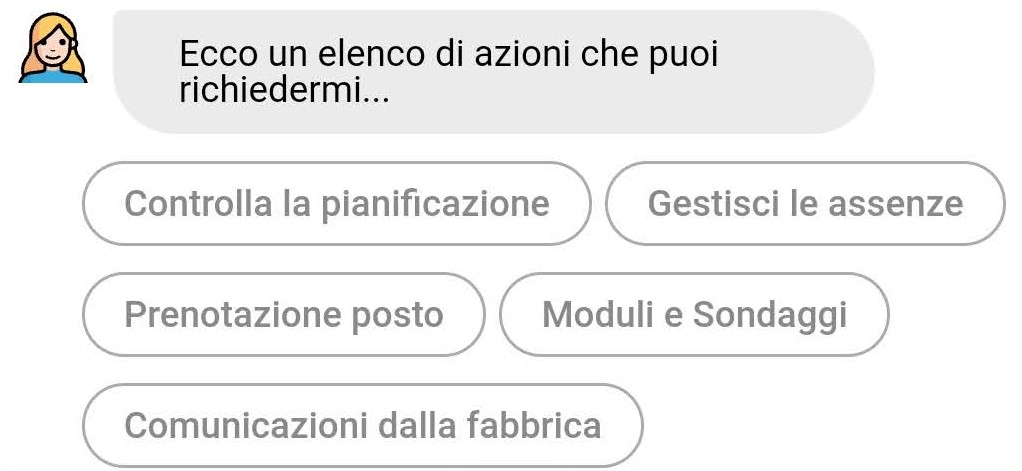
\includegraphics[scale=0.25] {blockItems.jpg}
	\caption{Esempio di messaggio prodotto da un blocco di tipo ASK}
\end{figure}

Oltre a campi del tipo \textbf{BLOCK} ha i seguenti campi in più:

\begin{itemize}
	\item \textbf{category}: Il blocco \textbf{ASK} è ulteriormente distinguibile in ASK o in MENU che si differenziano nel seguente aspetto:\\
	nel caso sia di categoria ASK tutte le opzioni disponibili portano a un blocco di conversazione successivo diverso mentre per MENU tutte le opzioni portano tutte allo stesso blocco;
	\item \textbf{source}: Parametro che contiene il nome di una variabile a cui fare riferimento per prendere i dati da utilizzare. Se non si fa riferimento a nessuna variabile allora va settato a \emph{NULL};
	\item \textbf{items}: Questo campo contiene un array d'oggetti di tipo \textbf{BlockItem} che rappresentano le possibile scelte che può fare l'utente, essi graficamente vengono rappresentati come dei pulsanti;
	\item \textbf{sourceType}: Parametro che indica la modalità di utilizzo della variabile contenuta nel campo \textbf{source};
	Ci sono solo due modalità disponibili:
	\begin{itemize}
		\item \textbf{LIST}: In questo caso la variabile contenuta in \textbf{source} viene ignorata e vengono presi tutti gli oggetti di tipo \textbf{BlockItem} contenuti nel campo \textbf{items} che vengono trasformati in bottoni da far visualizzare a video;
		\item \textbf{VARIABLE}: In questo caso tutto ciò che è contenuto nella variabile del campo \textbf{source} viene trasformato in bottoni da far visualizzare a video, per poterlo fare devono essere formattati in una struttura del tipo chiave valore.
	\end{itemize}	
\end{itemize} 

\subsubsection{SAY}

Il blocco di conversazione \textbf{SAY} ha la funzione di mostrare all'utente un messaggio a video attraverso il quale si comunica l'esito della operazione precedente e il risultato da essa ricavata. Perciò l'utente richiede l'esecuzione di una qualche operazione, viene eseguita e una volta conclusa il bot risponderà all'utente con il risultato ricavato precedentemente.

\begin{figure}[htbp]
	\centering
	
\includegraphics[scale=0.25]{say.jpg}
	\caption{DEsempio di messaggio prodotto da un blocco di tipo SAY}
\end{figure}
Oltre a campi del tipo \textbf{BLOCK} ha il seguente campo in più:

\begin{itemize}
	\item \textbf{attachment}: Campo che contiene un array d'oggetti di tipo \textsl{BlockAttachment} che permettono di allegare immagini o file PDF.
\end{itemize}

Inoltre sono presenti i campi \textbf{items}, \textbf{source} e \textbf{sourceType}, con analogo funzionamento del blocco \textbf{ASK} per inserire eventuali bottoni che aprono schede o link contenenti il risultato richiesto.

\subsubsection{IF}

Il blocco di conversazione \textbf{IF} ha la funzione di verificare se una o più condizioni sono rispettate. Perciò verifica se le condizioni sono soddisfatte, e in base all'esito verrà scelto il prossimo blocco da eseguire.

%\begin{figure}[htbp]
%	\centering
%	\includegraphics[scale=1]{img/if.png}
%	\caption{Definizione della classe IF}
%\end{figure}
Oltre a campi del tipo \textbf{BLOCK} ha i seguenti campi in più:

\begin{itemize}
	\item \textbf{conditions}: Contiene una o più condizioni che devono essere verificate;
	\item \textbf{trueBlockTarget}: Indica il blocco successivo da eseguire se le condizioni sono soddisfate;
	\item \textbf{falseBlockTarget}: Indica il blocco successivo da eseguire se le condizioni non sono soddisfate.
\end{itemize}


\subsubsection{PROC}
Il blocco di conversazione \textbf{PROC} permette di eseguire delle operazioni sulle variabili conversazionali cioè, assegnazione o trasformazione dei dati. Ad esempio, permette di riordinare i dati ricevuti dal server in modo da poter essere utilizzati dai \textbf{source} con \textbf{sourceType} uguale a \textbf{VARIABLE}.

%\begin{figure}[htbp]
%	\centering
%	\includegraphics[scale=1]{img/proc.png}
%	\caption{Definizione della classe PROC}
%\end{figure}

Oltre a campi del tipo \textbf{BLOCK} ha il seguente campo in più:

\begin{itemize}
	\item \textbf{expressions}: Contiene le espressioni da eseguire, ad esempio, per la formattazione dei dati.
	Ha i seguenti campi:
	\begin{itemize}
		\item \textbf{var}: Contiene il nome della variabile dove viene salvato il risultato della formattazione;
		\item \textbf{type}: Indica il tipo di formattazione che si vuole applicare, al momento c'è solo una formattazione disponibile:
		\begin{itemize}
			\item \textbf{reduce to textvalue}: Permette di riordinare i vari valori che si hanno in una struttura chiave valore.
		\end{itemize}
		\item \textbf{args}: Contiene un espressione in Handlebars, un linguaggio di \emph{templating} utilizzato per costruire \emph{template} in HTML con dei cosiddetti segnaposto che verranno poi valorizzati con dei valori, utilizzando delle \emph{keyword} del linguaggio, in modo da ottenere delle componenti in HTML da mostrare come messaggio.
	\end{itemize}
\end{itemize}

\subsubsection{JUMP}

Il blocco di conversazione \textbf{JUMP} permette di cambiare il flusso conversazionale ed eseguirne una altro. In termini tecnici si passa da un JSON di configurazione ad un altro dove ogni configurazioni in JSON contiene un specifico flusso di conversazione. Perciò, grazie a \textbf{JUMP} si può "saltare" da un flusso di conversazione a un altro.

%\begin{figure}[htbp]
%	\centering
%	\includegraphics[height=5cm]{img/jump.png}
%	\caption{Definizione della classe JUMP}
%\end{figure}

Nel campo \textbf{target} non viene indicato l'id del blocco successivo ma, l'id del \emph{flow} che si vuole eseguire.

\subsubsection{CALLFUNC}

Il blocco di conversazione \textbf{CALLFUNC} è il blocco attraverso il quale, il bot (l'applicazione mobile) può richiedere l’esecuzione di chiamate ad API (interne o esterne). Attraverso un WebSocket, che mantiene una connessione tra il bot e Azzurra.io, quest’ultima richiama, a sua volta, delle API di AWMS (o esterne ad AWMS) per ottenere i dati richiesti dell’utente o per salvare dati. 

%\begin{figure}[htbp]
%	\centering
%	\includegraphics[scale=1]{img/callfun.png}
%	\caption{Definizione della classe CALLFUNC}
%\end{figure}

Oltre a campi del tipo \textbf{BLOCK} ha il seguente campo in più:

\begin{itemize}
	\item \textbf{payload}: Campo che contiene l'intestazione e il corpo della richiesta verso Azzurra.io;
	Contiene i seguenti campi:
	\begin{itemize}
		\item \textbf{type}: Indica se la chiamata è verso Azzurra.io attraverso il valore \textsf{int} oppure verso un servizio esterno con il valore \textsf{ext}.
	\end{itemize}
	Se la chiamata è di tipo int ha la seguente struttura:
	\begin{itemize}
		\item \textbf{route}: Indica il metodo di Azzurra.io da richiamare;
		\item \textbf{body}: Contiene il corpo della richiesta, nello specifico un \emph{template} costruito da Handlebars che verrà idratato da Azzurra.io nel caso sia una richiesta di dati o dal bot nel caso in cui debba inviare dei dati da salvare.
	\end{itemize}
	Se la chiamata è di tipo ext ha la seguente struttura:
	\begin{itemize}
		\item \textbf{config}: Contiene la struttura di una chiamata HTTP.\\
		Ha i seguenti campi:
		\begin{itemize}
			\item \textbf{url}: Contiene l'indirizzo URL del servizio esterno a cui fare richiesta;
			\item \textbf{method}: Se la richiesta e di tipo GET o POST;
			\item \textbf{headers}: Contiene l'intestazione per la richiesta HTTP;
			\item \textbf{params}: Contiene le variabili necessarie per la chiamata, questo campo viene usato solo se la richiesta e di tipo GET;
			\item \textbf{data}: Analogo al campo \textbf{params} solo se viene usato dai metodi POST.
		\end{itemize}
	\end{itemize}
	\item \textbf{var}: Indica il nome della variabile dove salvare il risultato della richiesta;
	\item \textbf{failureBlockTarget}: Indica il blocco successivo da eseguire se la richiesta non va a buon fine;
	\item \textbf{successBlockTarget}: Indica il blocco successivo da eseguire se la richiesta va a buon fine.
\end{itemize}

\subsection{Oggetti ausiliari}
Come scritto nella sezione precedente questi oggetti vengono definiti per poterli utilizzare all'interno dei blocchi per svolgere un azione di supporto ai blocchi, affinché si possa raggiungere ciò per cui sono stati realizzati i blocchi di conversazione stessi.\\
\\
Di seguito vengono indicate tutte le classi degli oggetti ausiliari disponibili.

\subsubsection*{Widget}
È un oggetto che a seconda del tipo permette di realizzare delle componenti grafiche, esso viene utilizzo per richiedere delle azioni da parte dell’utente umano.
Ha i seguenti tipi:
\begin{itemize}
	\item \textbf{BUTTONS}: Genera dei bottoni arrotondati;
	\begin{figure}[h]
		\centering
		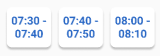
\includegraphics[scale=1.1]{buttons.png}
	\caption{Rappresentazione grafica dei buttons}
	\end{figure}
	\clearpage
	\item \textbf{ITEMS}: Genera dei bottoni quadrati;
	\begin{figure}[h]
		\centering
		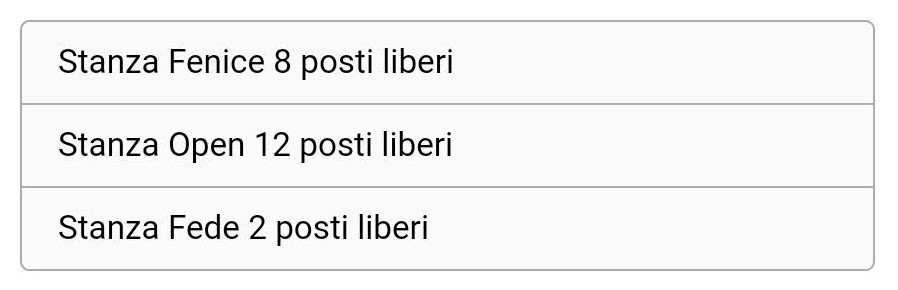
\includegraphics[scale=0.3]{items.jpg}
		\caption{Rappresentazione grafica degli items}
	\end{figure}
	\item \textbf{PICKER}: Genera attraverso l'ion-picker di \textsf{Ionic} una finestra di dialogo dove si può selezionare una opzione tra quelle proposte;
	\begin{figure}[h]
		\centering
		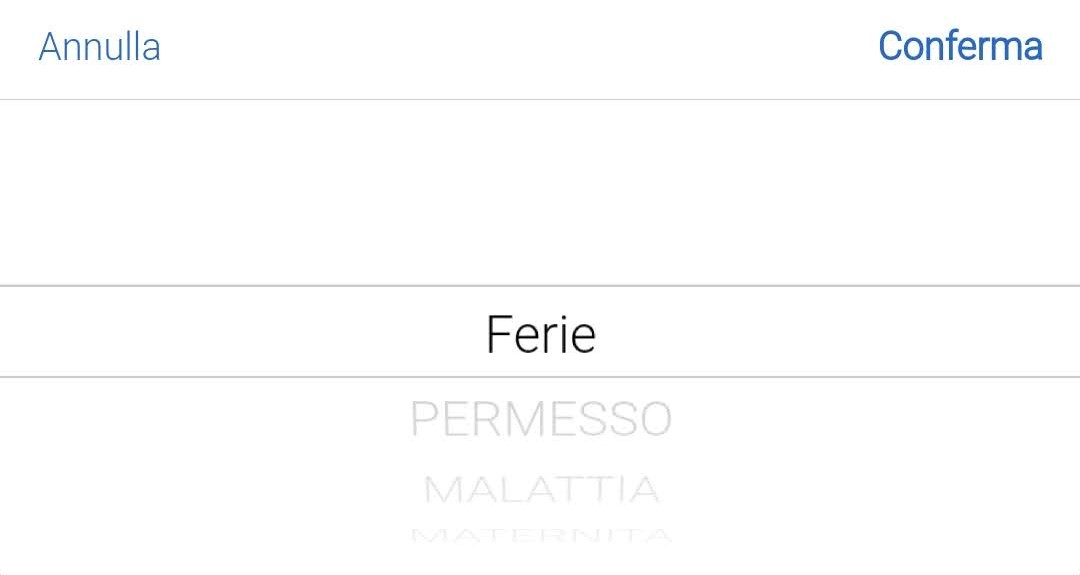
\includegraphics[scale=0.2]{picker.jpg}
		\caption{Rappresentazione grafica del picker}
	\end{figure}
	\item \textbf{TIMEPICKER}: Analogo al \textbf{PICKER} solo che le opzioni da scegliere e l'orario che si vuole selezionare;
	\begin{figure}[h]
		\centering
		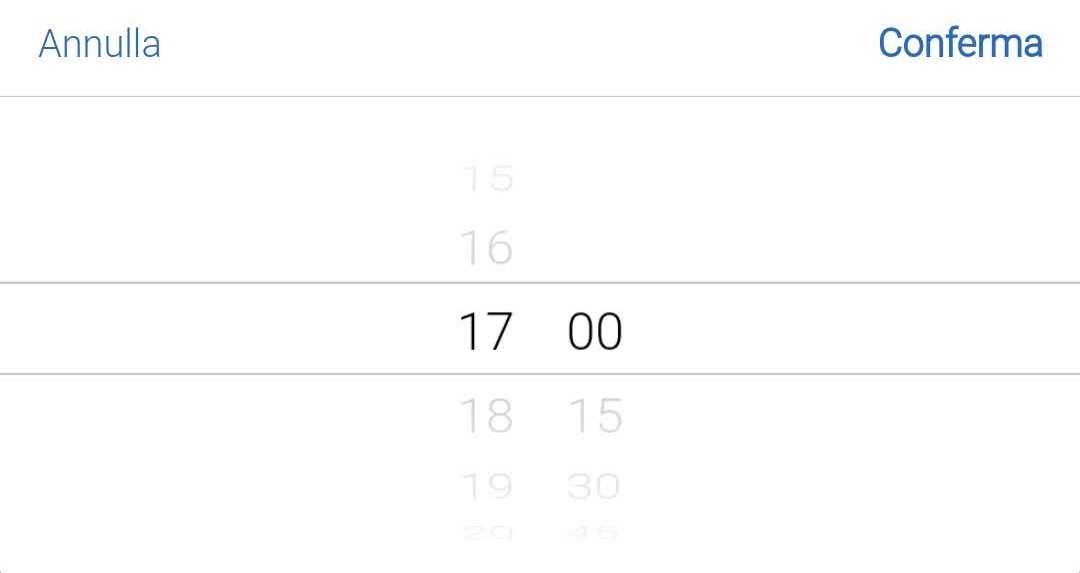
\includegraphics[scale=0.2]{timePicker.jpg}
		\caption{Rappresentazione grafica del time picker}
	\end{figure}
\clearpage
	\item \textbf{DATEPICKER}: Analogo al \textbf{PICKER} solo che le opzioni da scegliere e la data che si vuole selezionare;
	\begin{figure}[h]
		\centering
		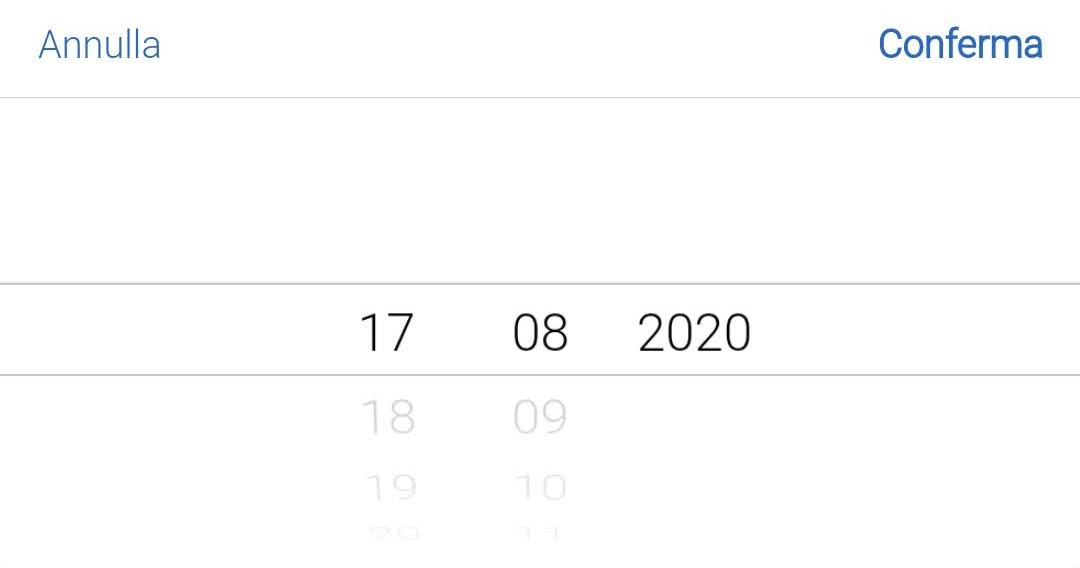
\includegraphics[scale=0.2]{datePicker.jpg}
		\caption{Rappresentazione grafica del date picker}
	\end{figure}
	\item \textbf{CALENDAR}: Fa comparire un calendario grazie all'utilizzo del plugin Calendar per Ionic;
	\item \textbf{QRSCANNER}: Permette di accedere alla fotocamera (solo se si hanno i permessi) e leggere i codici \textsf{QR-code} tutto ciò grazie al plugin QR Scanner per Ionic.
	\begin{figure}[h]
		\centering
		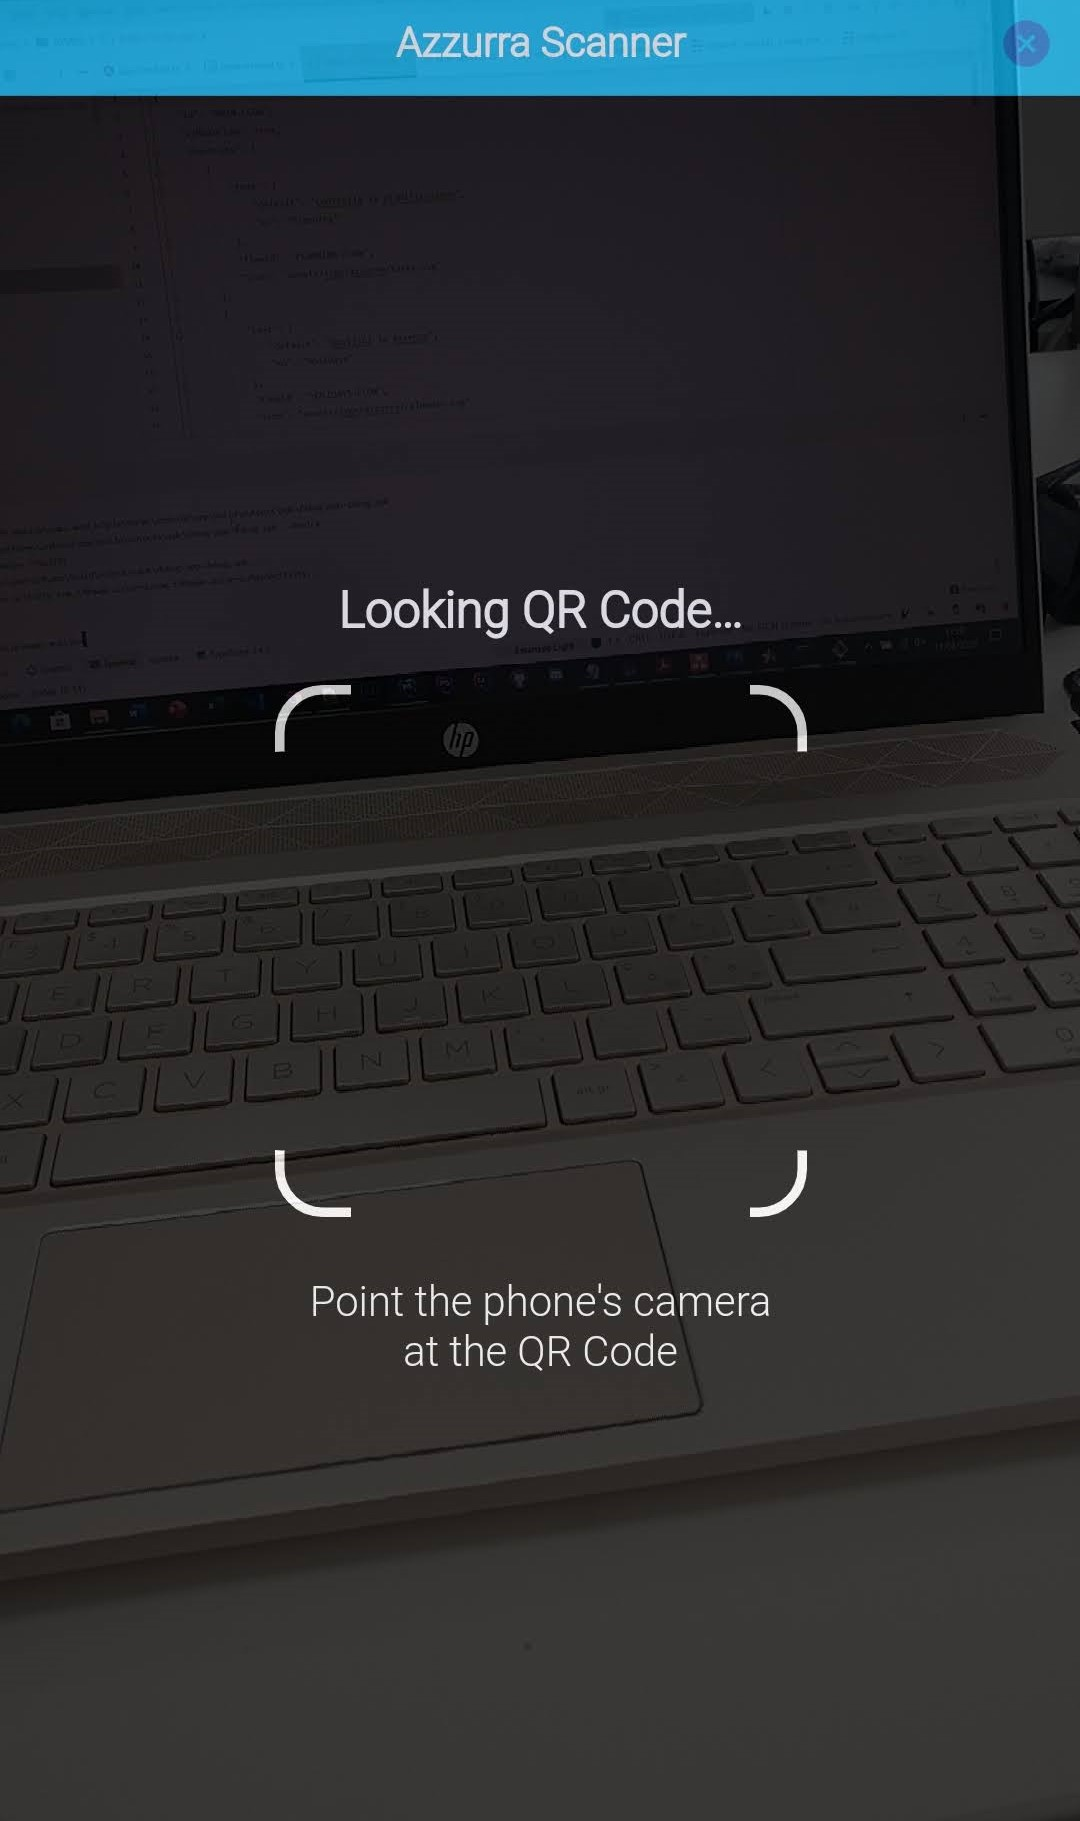
\includegraphics[scale=0.2]{qrcode.jpg}
		\caption{Rappresentazione grafica del QR scanner}
	\end{figure}
\end{itemize}

\subsubsection*{BlockItem}
Questo oggetto rappresenta una possibile scelta che può fare l'utente, graficamente viene rappresentato come un bottone cliccabile dall'utente.

\begin{figure}[h]
	\centering
	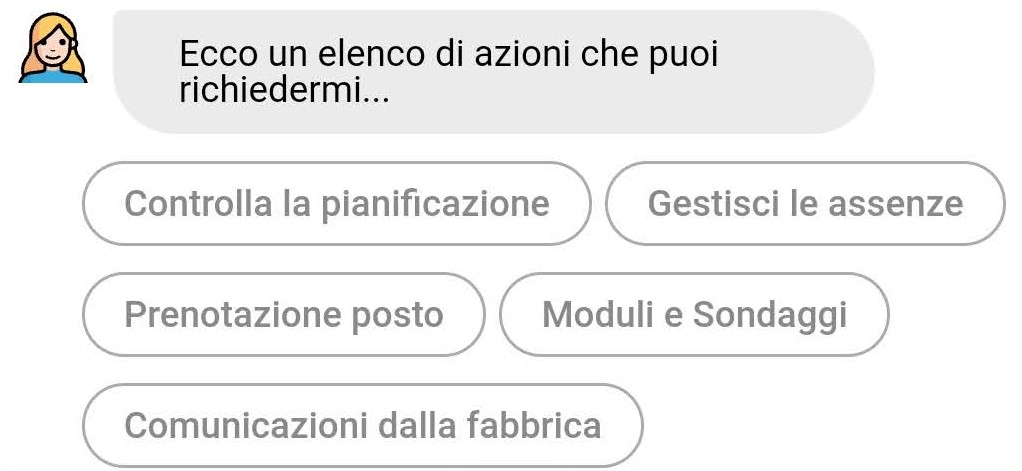
\includegraphics[scale=0.3]{blockItems.jpg}
	\caption{Rappresentazione grafica del BlockItem}
\end{figure}
Ha la seguente struttura:

\begin{itemize}
	\item \textbf{text}: Contiene l'etichetta che viene visualizzata sul bottone;
	\item \textbf{target}: Contiene l'id del prossimo blocco da eseguire.
\end{itemize}



\subsubsection*{BlockAttachment} 
L'oggetto in esame permette di allegare immagini o file PDF da mostrare all'utente.

Ha la seguente struttura:

\begin{itemize}
	\item \textbf{id}: Contine un codice univoco che identifica ogni \textsl{BlockAttachment};
	\item \textbf{type}: Indica se contiene un PDF o una immagine, nel caso di un'immagine indica se è in formato JPG o in JPEG oopure in PNG.
\end{itemize}	

\section{Funzionamento di Azzurra Flow Engine}
Come detto il \textbf{Azzurra Flow Engine} è l'elemento in grado di interpretare i dati contenuti nelle configurazioni JSON. Grazie a ciò è possibile eseguire il corretto flusso della conversazione e generare i messaggi della conversazione. 
\subsection{Messaggio del bot Azzurra}
Per implementare le funzionalità del \textbf{Azzura Flow Engine} vengono utilizzati:
\begin{itemize}
	\item \textbf{FlowService}: Ha i metodi necessari per interpretare le configurazioni JSON e quindi, per poter sapere quale tipo di messaggio deve essere costruito, ricavare i dati necessari per costruire i messaggi e sapere come procedere con la conversazione;
	\item \textbf{AzzurraService}: Permette principalmente di fare da tramite tra il \textbf{FlowService} e il \textbf{ChatComponent} per la creazione della conversazione. Oltre a ciò permette di gestire operazioni ad alto livello come il caricamento dei messaggi precedenti nel chat e gestire le notifiche che possono arrivare dalla \emph{dashboard};
	\item \textbf{ChatComponent}: Si occupa di far visualizzare i messaggi della conversazione;
	\item \textbf{ChatService}: Ha il compito di creare e gestire i Widget da aggiungere al messaggio da mostrare, e inoltre, di ricavarne da essi le risposte dell'utente umano.
\end{itemize}

\begin{figure}[htbp]
	\centering
	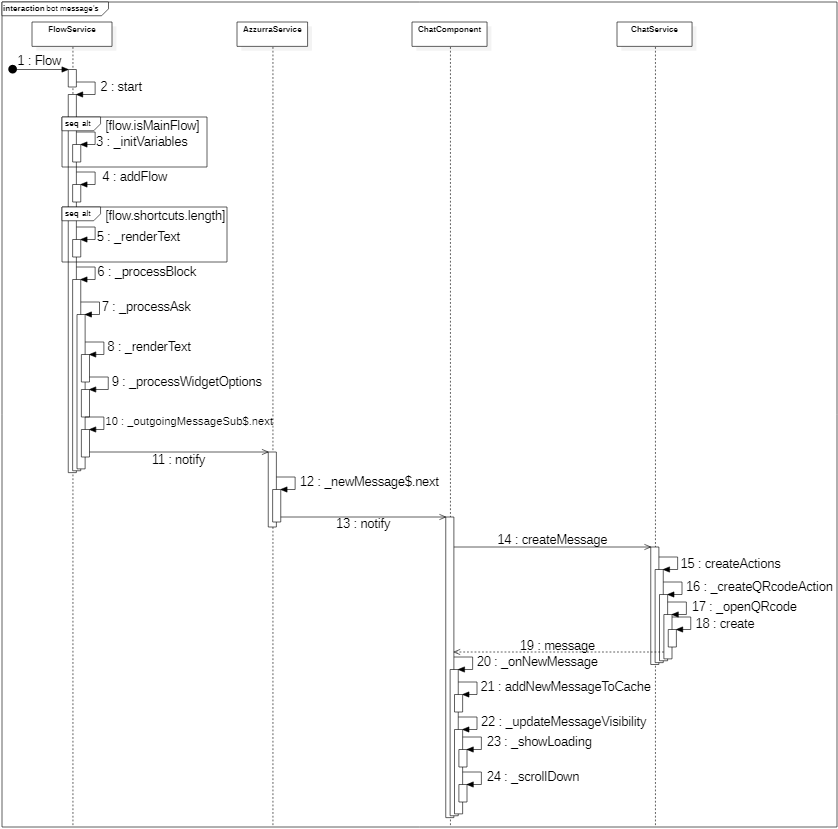
\includegraphics[height=20cm, width=14cm]{sd_bot_mx2.png}
	\caption{Diagramma di sequenza del processo di generazione del messaggio del bot Azzurra}
\end{figure}
Una volta che si è stabilità la connessione con \textbf{Azzurra.io}, attraverso un \gls{WebSocket}, inizializzato il \textbf{Flow Engina} e infine, ricevuto la configurazione JSON contenente il flusso conversazionale, la generazione di un messaggio da parte del bot Azzurra prevede i seguenti passi:\\
\begin{enumerate}
	\item Viene inviato alla applicazione mobile il flusso conversazionale richiesto precedentemente;
	\item Viene avvitato nel \textbf{FlowService} il metodo \textbf{start()} il quale riceve in input il flusso da eseguire. Viene verificato se il flusso ricevuto risulta essere il \emph{main flow}, in questo caso vengono inizializzate le variabili conversazionali d'ambiente utilizzate come supporto per la generazione dei messaggi, ad esempio esiste una variabile d'ambiente per indicare il giorno corrente o il formato della data da utilizzare;
	\item Una volta impostate le variabile ambiente, usciti dal blocco condizionale, viene salvato il flow da eseguire attraverso il metodo \textbf{\_addFlow()} che inoltre, imposta come flusso corrente da eseguire il flusso ricevuto in input;
	\item All'interno del metodo \textbf{\_addFlow()} viene controllato se la configurazione definisce delle eventuali \textbf{shortcuts}
	\item Se ci sono delle \textbf{shortcuts} viene chiamato il metodo \textbf{\_renderText()} per crearle, esso sarà in grado di interpretare il pezzo di configurazione dove sono definite le proprieta di ogni \textbf{shortcuts}.\\
	
	Una volta finita l'esecuzione del metodo, l'esecuzione torna nel metodo \textbf{start()}\\
	\item Sempre nel metodo	\textbf{start()} viene chiamata l'esecuzione del metodo \textbf{\_processBlock()} dandogli in input il primo blocco del flusso da eseguire
	
	\item Nel metodo \textbf{\_processBlock()} viene eseguito il blocco che riceve in input, in questo caso il blocco da eseguire è il primo blocco del flusso come detto nel punto precedente. In questo metodo si verifica innanzitutto se c'è un blocco da eseguire, se non c'è viene emesso un segnale che informa che il flusso di conversazione è terminato, mentre se c'è un blocco allora si imposta questo blocco come quello in esecuzione e si verifica di che tipo è il blocco.\\
	A seconda del tipo del blocco esegue le seguenti istruzioni:
	\begin{itemize}
		\item \textbf{Caso SAY}: Viene eseguito il metodo \textbf{\_processSay} dandogli in input il blocco corrente. Il metodo prende il valore salvato nel campo \textbf{text} e le eventuali \textbf{variations} del blocco generando il testo messaggio da mostrare attraverso il metodo \textbf{\_renderText()}. Vengono generati eventuali items attraverso il metodo \textbf{\_buildSayItems()} il quale controlla il sourceType e in base al valore che ha, genera gli items. Tornando in \textbf{\_processSay}, se presenti vengono anche eseguite le \textbf{widgetOptions} attraverso il metodo \textbf{\_processWidgetOptions()} e creati gli eventiali \textbf{BlockAttachment}. Infine, viene emesso il nuovo messaggio creato per il bot Azzurra e si passa all'esecuzione del prossimo blocco;
		\item \textbf{Caso ASK}: Viene eseguito il metodo \textbf{\_processAsk} dandogli in input il blocco corrente. Il metodo salva il nome della variabile contenuta nel campo \textbf{var}, che contiene la risposta dell'utente. Analogamente per quanto accede per il blocco \textbf{SAY} viene creato il testo della domanda e attraverso il metodo \textbf{\_buildQuestions} vengono creati gli items delle possibili scelte. Inoltre, vengono processati gli eventuali \textbf{widgetOptions} e create le varie opzioni di scelta. Infine, viene emesso il nuovo messaggio creato per il bot, il quale rimane in attesa della risposta dell'utente umano quando verrà visualizzato il messaggio;
		\item \textbf{Caso JUMP}: Richiama il metodo \textbf{\_getFlow()} per prendersi l'identificativo del flusso da eseguire attraverso la lettura del campo \textbf{target}. Il metodo citato richiede ad Azzurra.io il flusso che ha l'identificativo ricevuto in input, e una volta ricevuto ricomincia l'esecuzione del flusso conversazionale richiamando il metodo \textbf{start()};
		\item \textbf{Caso IF}: Valuta la condizione se vera o falsa, in base a ciò stabilisce quale sarà il blocco di conversazione successivo;
		\item \textbf{Caso PROD}: Stabilisce che formattazione deve essere fatta, richiama il metodo corretto per farla e poi passa all'esecuzione del prossimo blocco;
		\item \textbf{CALLFUNC}: Viene ricavato il payload del blocco, viene codificato il template in handlebars per generare il corpo della richiesta, una volta fatto ciò la richiesta è pronta e viene mandata a \textbf{Azzurra.io}. Successivamente viene salvata la risposta sulla variabile indicata del campo \textbf{var} e in base alla risposta, se andata a buon fine oppure no, si eseguirà il corrispondente blocco successivo.
	\end{itemize}
\end{enumerate}
 
  




Nel \textbf{AzzuraService} c'è un ascoltatore che riceve i segnali mandati dai metodi di \textbf{FlowService}, grazie a ciò \textbf{AzzuraService} ha sempre il nuovo messaggio creato. Ora che il messaggio è stato creato bisogna poterlo visualizzare nella UI, più precisamente nella chat tra il bot Azzurra l'utente umano, per farlo \textbf{AzzuraService} emettere a sua volta il nuovo messaggio che è stato creato, verso l'ascoltatore presente in \textbf{ChatComponent}. Quando \textbf{ChatComponent} riceve il messaggio eseguirà il metodo \textbf{createMessage()} di \textbf{ChatService} passandogli il messaggio ricevuto.\\ Questo metodo si occuperà di far creare il messaggio grafico nel modo corretto. Innanzitutto verifica chi ha emesso il messaggio, l'utente umano o bot Azzurra. Nel caso in cui il messaggio sia del bot Azzurra viene indicato il testo da mostrare estraendolo dal messaggio ricevuto in input, aggiunto lo sprite di Azzurra per indicare graficamente che il messaggio viene dal bot.
\\
Nel caso in cui il messaggio preveda delle azioni da parte dell'utente umano, ovvero ci siano dei \textbf{Widget}, viene chiamato il metodo \textbf{createAction()} passandogli sempre il messaggio. In questo metodo viene verificato che tipo di \textbf{Widget} deve essere creato, per ogni \textbf{Widget} c'è un corrispondente metodo che ne imposta il testo da far visualizzare quando l'utente interagisce con esso, tale testo potrebbe essere un testo di default o un testo indicato nel campo \textbf{widgetOptions} inoltre nel caso del \textbf{DATEPICKER} o \textbf{TIMEPICKER}, viene impostato il formato di visualizzazione del giorno e dell'ora. Successivamente viene richiamato il metodo attraverso il quale le componenti di \textbf{Ionic} creano graficamente il \textbf{Widget} necessario, il quale alla fine della creazione viene ritornato al \textbf{ChatComponent}.
\\
Il messaggio ora appare nella UI, nella chat con il bot Azzurra. Per tenere uno storico sulla chat di tutti i messaggi inviati si richiama il metodo \textbf{addNewMessageToCache()} del \textbf{DataSourceService}, dandogli il nuovo messaggio. \\
\\
Una volta che l'utente interagisce con il \textbf{Widget} deve essere creato il messaggio dell'utente umano con la sua risposta. 

\pagebreak


\subsection{Messaggio dell’utente  umano}
La generazione di un messaggio da parte dell’utente  umano prevede le seguenti azioni:\\
Quando l'utente esegue un'azione che genera la risposta il \textbf{ChatService} emette il valore della risposta ogni volta che un \textbf{Widget} riceve la risposta. Nel \textbf{ChatComponent} esiste un ascoltatore per ogni evento emesso da ogni \textbf{Widget}, quando viene ricevuto il messaggio con la risposta dell'utente viene chiamato il metodo di \textbf{AzzurraService}, \textbf{sendReply()} dandogli in input il messaggio di risposta solo se il messaggio è valido, se non lo è viene ignorato.
\\
Il metodo \textbf{sendReply()} chiama a sua volta il metodo \textbf{processHumanAction} di \textbf{FlowService} dove in questo metodo viene impostato il valore della risposta dell'utente nella variabile indicata nel campo \textbf{var}, dopo di che si verifica se \textbf{Widget} abbia al suo interno un proprio campo target, se sì viene impostato come prossimo blocco di conversazione il blocco che il codice identificativo uguale a quello contenuto nel target, se invece non ha un campo target proprio si va a prendere il valore del campo target del blocco e si imposta il suo valore come prossimo blocco da eseguire. 
\\
Impostati tutti i dati necessari occorre presentare il messaggio nella UI, viene perciò emesso il messaggio dell'utente umano. Il messaggio viene nuovamente catturato da AzzurraService e inviato a ChatComponent dove vengono rifatte le stesse operazioni che erano state fatte per il messaggio del bot Azzurra solo che nel metodo \textbf{createMessage()} di \textbf{ChatService} verrà creato un messaggio di un utente umano ritornandolo al \textbf{ChatComponent} che si occuperà di farlo visualizzare.

\begin{figure}[htbp]
	\centering
%	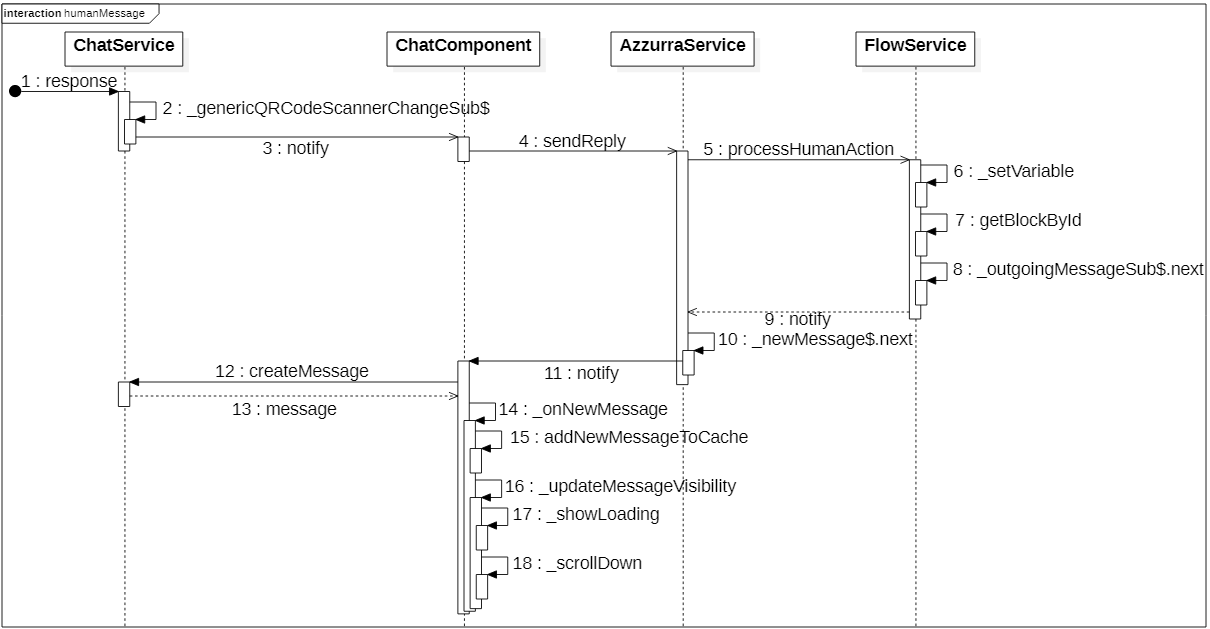
\includegraphics[scale=0.71]{sd_human_mx.png}
	\caption{Diagramma di sequenza del processo di generazione del messaggio del bot Azzurra}
\end{figure}